%!TEX root = ../dissertation.tex
\begin{savequote}[75mm]
The Secret of Happiness lies in looking at all the wonders of the world and never forgetting the two drops of oil in the spoon.
\qauthor{The alchemist, Paulo Coelho}
\end{savequote}

\chapter{Materials and methods}

\section{Shell fabrication}
\subsection{Motivations}
\paragraph{}
This study requires a full control over the geometry, the material and the manufacturing process to ensure the reproducibility of the experiments.\\
Further more, two constraints were to take into account: the ability to induce the buckling within a pressure range of -1 bar and 1 bar and the ability to apply several cycles without damaging the shell. 
\paragraph{}This implies that the material to be used needs to have a high tensile strength to withstand the deformation cycle without entering the plastic domain and a rigidity small enough to trigger a buckling in the imposed pressure range and a feasible $(\frac{d}{R})$ range i.e $d > 1 mm$ and $R < 50 mm$. Visco-elastic polymers called elastomers qualify to these prerequisites and have been chosen for the shell manufacturing.
\subsection{Why in-situ molding}
\paragraph{}
Before deciding to manufacture spherical hollow shells, we tried different kind of commercial "`balls"'. It was not conclusive because the process of fabrication was not intended to be reproducible in terms of material composition, thickness or diameter. This is why it was decided to manufacture them.

\paragraph{}
Several techniques were considered to manufacture polymer-based spherical hollow shells, including 3D-printing, rotational molding, processes involving high-pressure vulcanization. These techniques would have required either buying expensive equipments or subcontracting to a company with inconveniences of time delay, loss of control over the process and expensive cost of prototyping. 
The most suitable solution was the more common bi-molding process where the two halves of an object are cast and then assembled. The main advantages being the cost and the low-time consumption, plus a total control over the process, which includes the choice of materials, the reproducibility and more freedom over the geometry.
\subsection{Molding process}
\subsubsection{Molding equipments}
\paragraph{Female mold:}
It consists of a cylinder of radius $R_{cylinder}=30 mm$  hollowed out to produce a half a sphere imprint of radius $R_{out}=25 mm$ and a height of $h = 30 mm$ (see fig.\ref{fig:female_mold}). The concavity is where the casting material is poured.
A groove was added to store any potential material surplus. Two female molds are necessary for the casting operation.
\begin{wrapfigure}{r}{0.5\textwidth}
  \begin{center}
    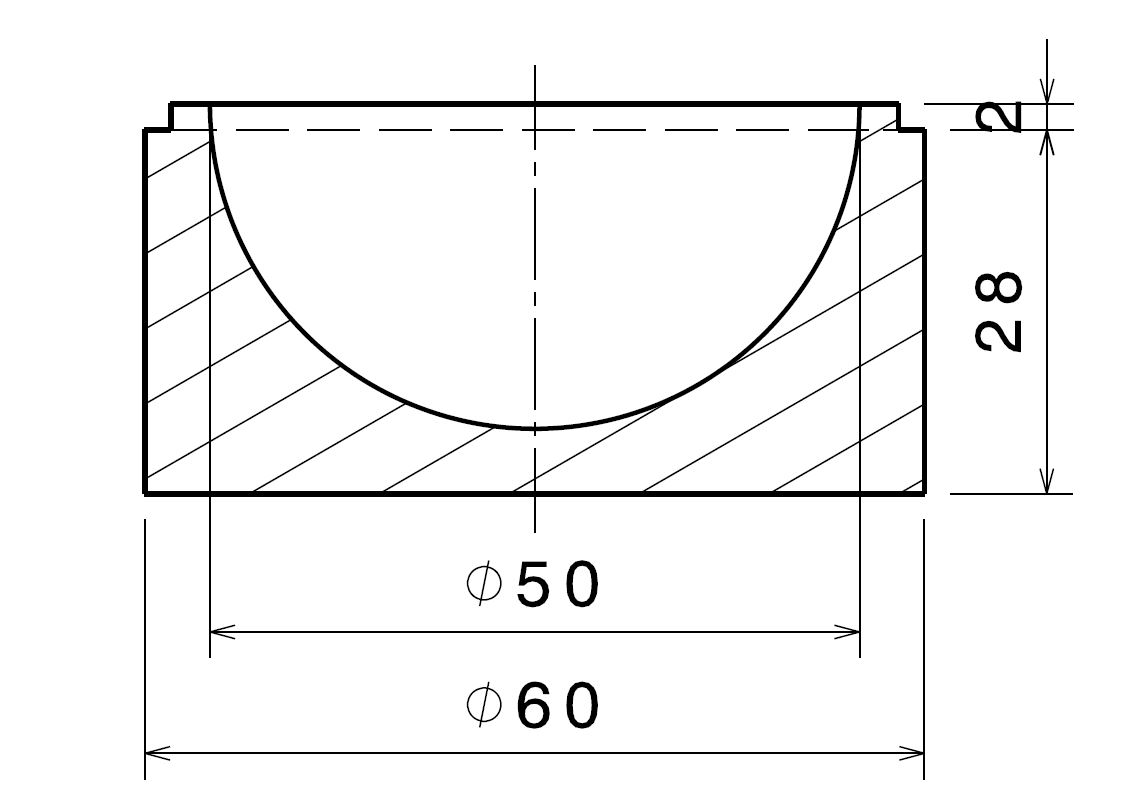
\includegraphics[width=0.48\textwidth]{figures/Chapter_1/female_mold.png}
  \end{center}
	\label{fig:female_mold}
  \caption{longitudinal section of the female mold}
\end{wrapfigure}%
\paragraph{Translation guide sleeve:}
It is a hollow cylinder with an inner radius $R_{in} = R_{cylinder} = 30 mm$, and a thickness of $5 mm$. where the female mold is slid in. It is slightly higher than the female mold by $5 mm$. One extremity is provided with an inner chamfer of $5°$ which ensures the concentricity between the female mold and the male mold.
\begin{wrapfigure}{r}{0.5\textwidth}
  \begin{center}
    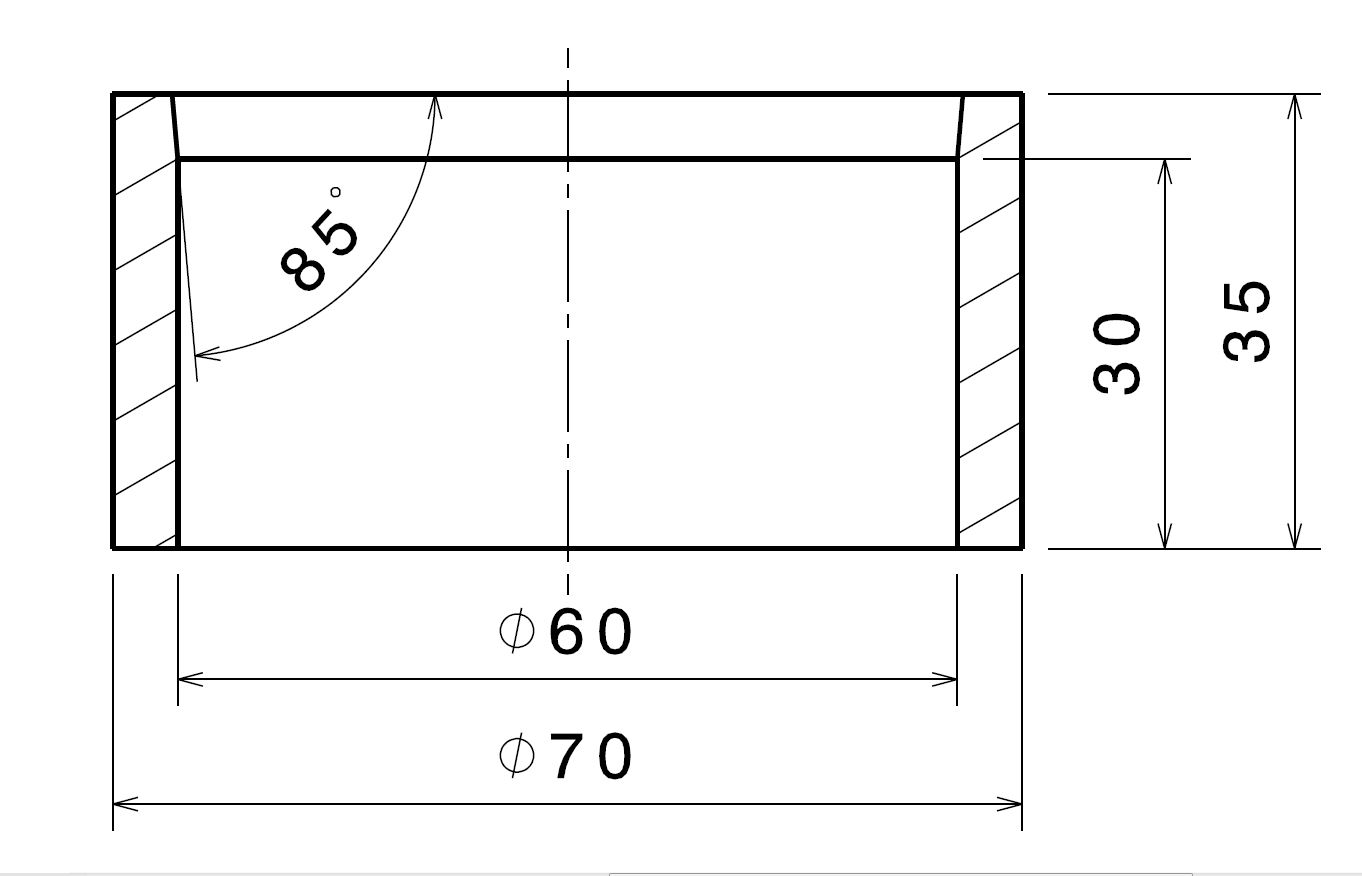
\includegraphics[width=0.48\textwidth]{figures/Chapter_1/sleeve_translation.png}
  \end{center}
	\label{fig:sleeve_1}
  \caption{longitudinal section of the sleeve}
\end{wrapfigure}%
\paragraph{Male mold:}
Figure \ref{fig:male_mold} shows the design of the male mold which consists of half a sphere of radius $R_{int}<R_{out}$, which is changed to cast different thicknesses. It is supplied with a shouldering which acts as a travel stop, its flanks have a slight angle of 5 providing a translation guide and preventing an over-center locking in combination with the guiding sleeve previously presented. The cylindrical part over the shouldering helps manipulating the mold during the casting process. Three radii have been used: $R_{int} = 18.5 mm, 20 mm, 23 mm$. 
\footnote{All the molding parts presented are made of Aluminium "`Fortal"'. The female and male molds were machined using a CNC (computerized numerical control)  machine and with a precision of $tol =\pm 0.01 mm$. The surface roughness obtained was of $R_a = 0.04$ which indicates a very good finishing.
This choice of manufacturing was unavoidable since no other alternative could produce spherical shapes with such precision conditions.}
\begin{wrapfigure}{r}{0.5\textwidth}
  \begin{center}
    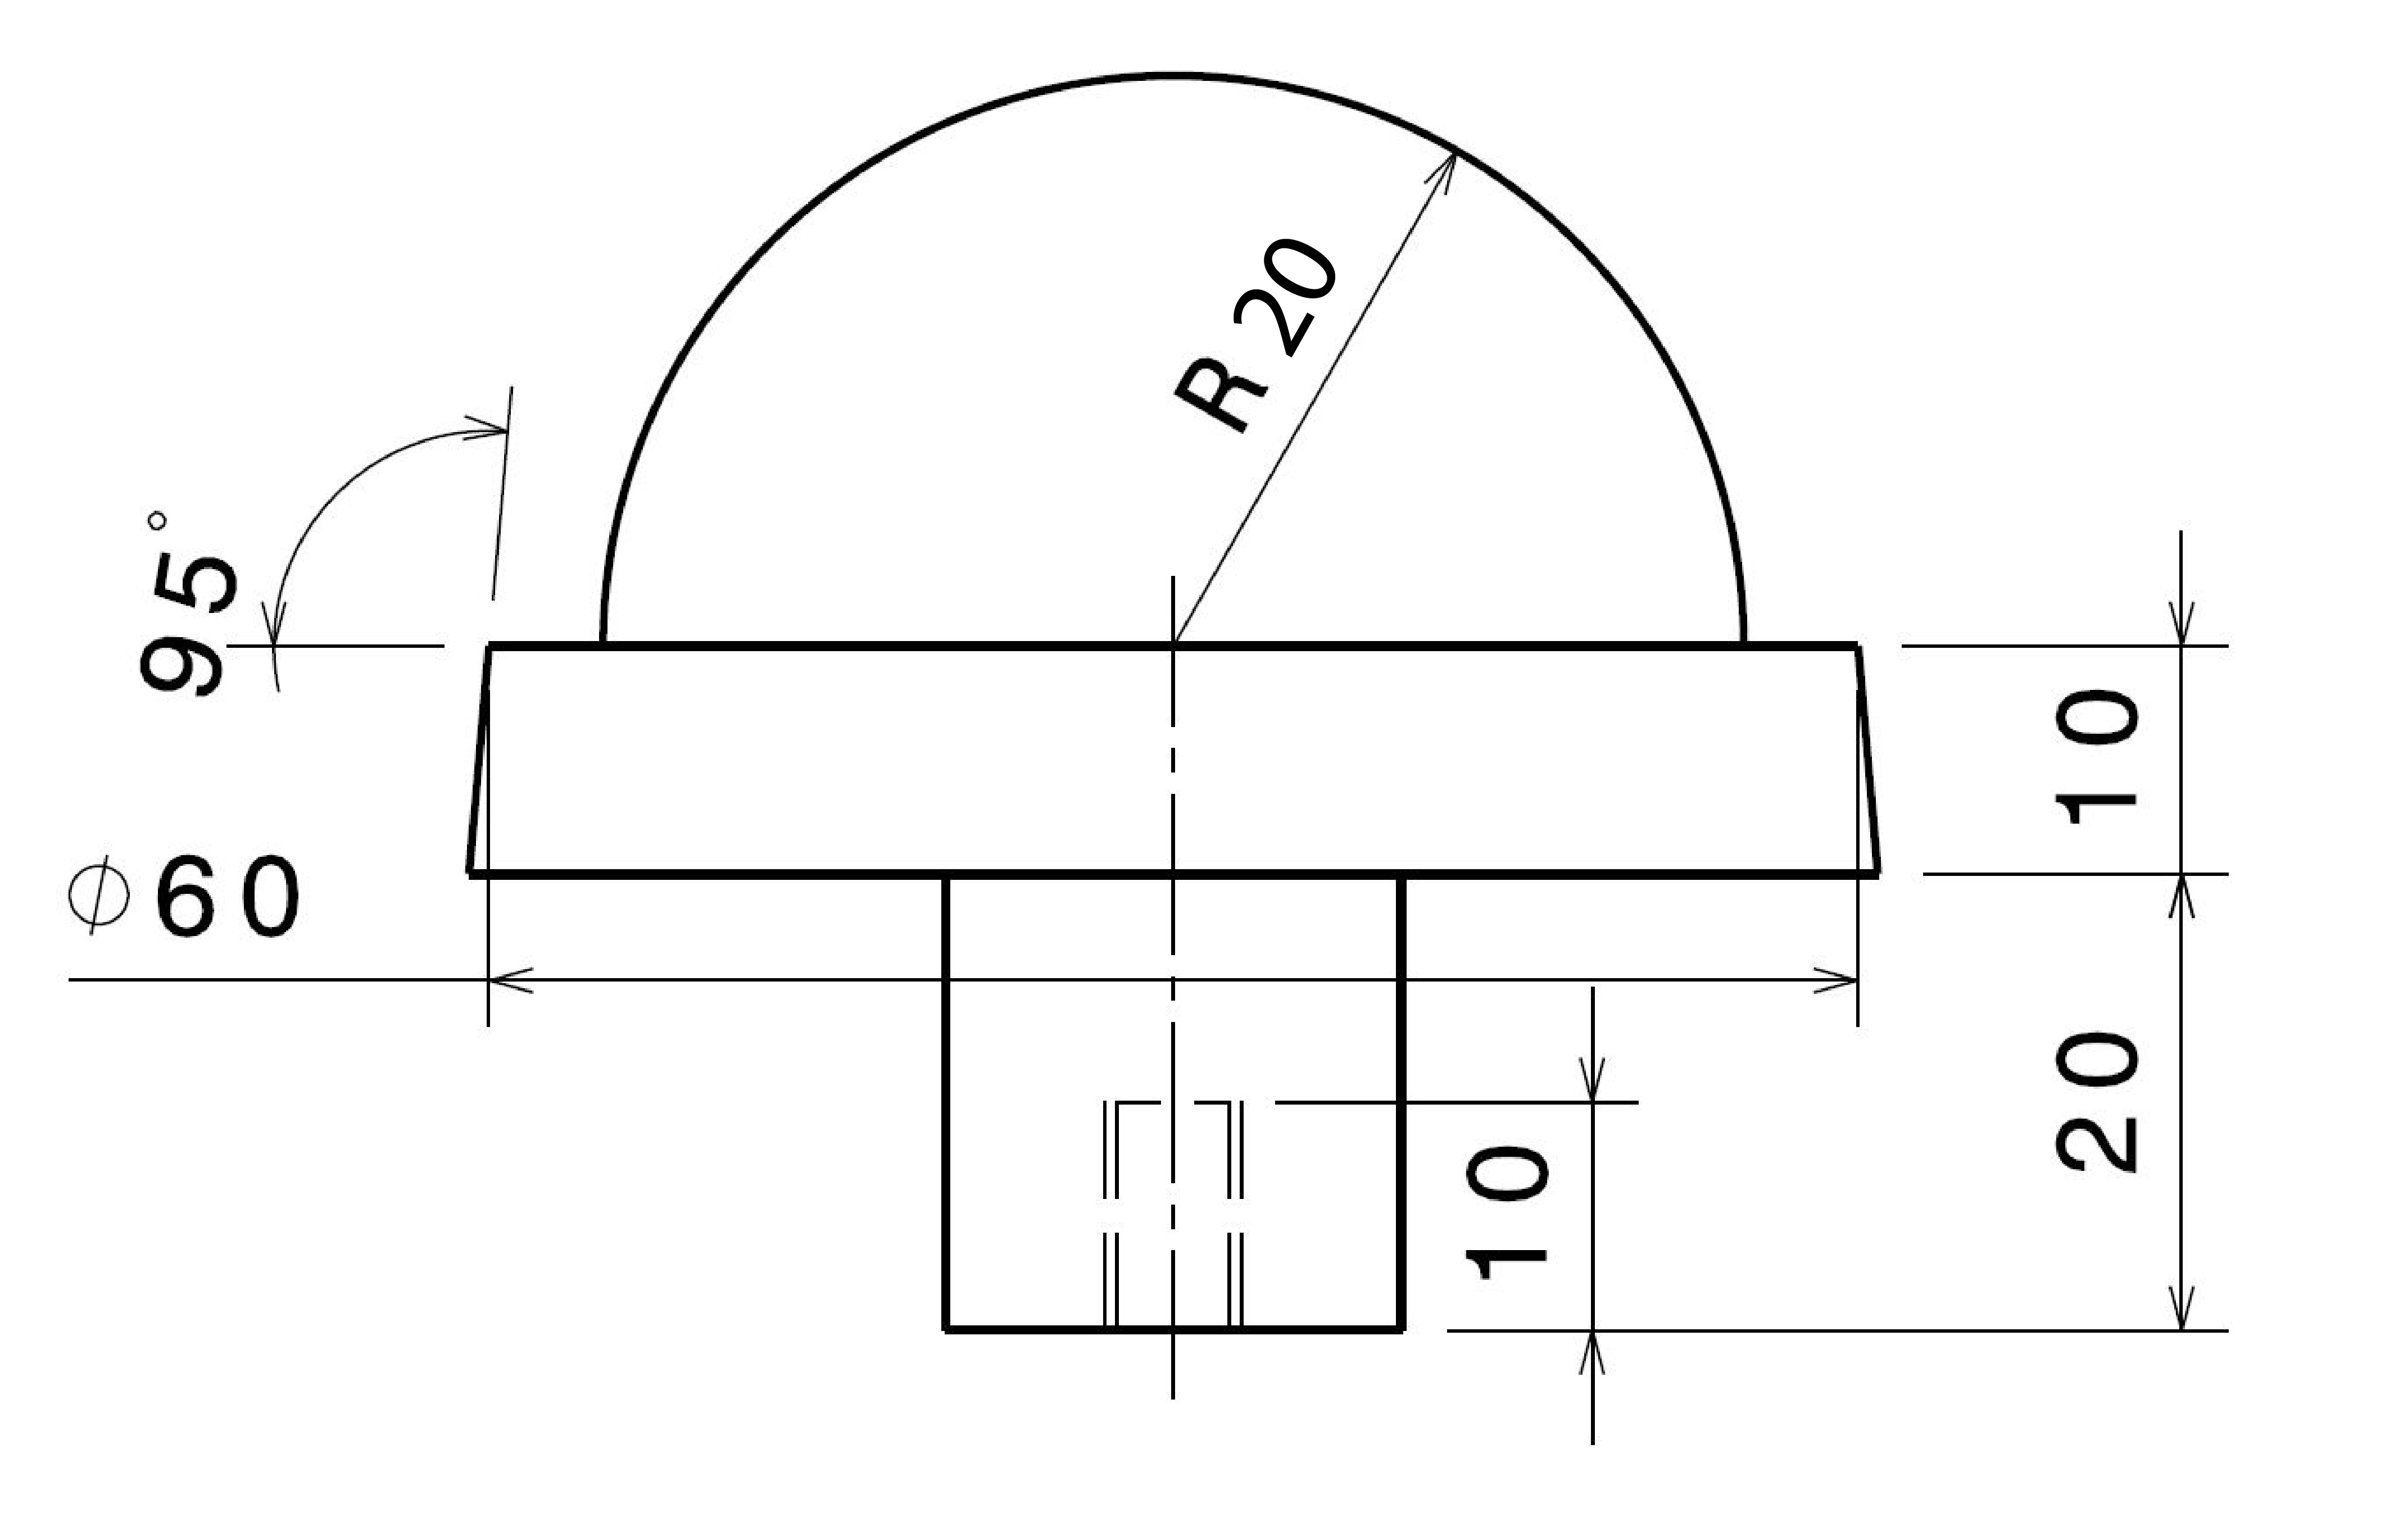
\includegraphics[width=0.48\textwidth]{figures/Chapter_1/male_mold.png}
  \end{center}
	\label{fig:male_mold}
  \caption{longitudinal section of the male mold}
\end{wrapfigure}%
\paragraph{Gluing sleeve}
It is a hollow cylinder with an inner radius $R_{in} = R_{cylinder} = 30 mm$, a thickness of $5 mm$ and a height of $50 mm$. It is used during the gluing process to ensure the concentricity of the two halves of the sphere contained in the female molds which face each other.
\paragraph{Mechanical press}
It's a simple press consisting of two metallic plates supplied with a set of threaded rods and hexagonal nuts used to apply pressure over female/male molds during the casting step to prevent bubbles from appearing during the casting step. It is also used during the gluing step on the female/female molds to ensure the contact between the two half spheres to be glued together.
\subsubsection{Materials}
\paragraph{}
Three materials were used in the experiments done during the study.\\ 
\paragraph{Dragon skin 30}
This material is typically used to make special effects.In the case of our study, it was used to investigate the effect of the $\frac{d}{R}$ on the swimming mechanism. Its exact chemical constitution is not known, but what can be said is that it is cure liquid silicone compound, which consists of two liquid components named A and B. Component \emph{A} represents the silicon polymer chains with eventually the presence of fillers to enhance its mechanical properties. Component \emph{B} is the cross-linking agent providing bonds that link one polymer chain to another, decreasing the flexibility of the polymer chain and increasing its rigidity. Mixing these two components at room temperature, it creates a solid that takes the shape of the container it was poured in.
The typical mechanical properties of the resulting rubber are:
\begin{itemize}
	\item[Shore A Hardness]: 30 
	\item[Specific gravity]: 1.08 
	\item[100\% elastic modulus]: 0.6 MPa
	\item[Elongation at break]: 364\%
	\item[cure time (at room temperature)]: 16 hours
\end{itemize}

\paragraph{}
The two remaining materials \emph{AJO 121} and \emph{AJO 122} were samples kindly supplied by \emph{BLUESTAR silicon}.Both are hot curing silicone rubbers after addition of a vulcanization agent, in this case it is 1.25 \% of \emph{2,4-dichlorobenzoyl peroxide}. They were chosen to investigate the effect of solid dissipation characterized by the rebound resilience property. This pair of materials present the particularity of sharing the same elastic energy storage capacity characterized by the elastic modulus. The vulcanization process is temperature-controlled and is induced at 110°C.
The typical mechanical properties of the resulting rubbers are:
\begin{itemize}
	\item[100\% elastic modulus AJO121 / AJO122]: 2.2 MPa / 2.3 MPa
	\item[Rebound resilience AJO121 / AJO122]: 45\% / 65\%
	\item[Shore A AJO121 / AJO122]: 60 / 59 
	\item[Specific gravity]: 1.16
	\item[Elongation at break AJO121 / AJO122]: 560\% / 366\%
	\item[cure time (at 115°C)]: 10 minutes
\end{itemize}


 


\subsubsection{}
